\section{Passive Elemente}
\subsection{Lernziele}
\begin{itemize}
  \item Widerstände: Typen und Grössen
  \item Kondensatoren: Typen und Vor- und Nachteile
  \item Induktivitäten
\end{itemize}

\subsection{Widerstände}
\subsubsection{Kenngrössen}
\begin{itemize}
  \item Widerstandswert
  \item Toleranz des Widerstandswertes (Anliefertoleranz)
  \item maximale Verlustleistung
  \item maximale Oberflächen- oder Filmtemperatur
  \item Temperaturkoeffizient (TK-Wert, angegeben in der Form TKxxx mit xxx = ppm pro Kelvin)
  \item Spannungsfestigkeit
  \item Langzeitstabilität (Drift) bei maximaler Verlustleistung\\
  Nennleistung über die Lebensdauer
  \item parasitäre Induktivität
  \item parasitäre Kapazität
  \item Stromrauschen
  \item Impuls-Belastbarkeit (kurzzeitige Überbelastbarkeit)
\end{itemize}

\subsubsection{Kriterien, Einteilung}
\begin{itemize}
  \item Bauform
  \item Leistung
  \item Widerstandsmaterial
  \item Anforderungen an die Genauigkeit und Langzeitstabilität
  \begin{itemize}
    \item Präzisionswiderstand (< 0,1 \%, in analogen Schaltungen mit Opamps)
    \item Messwiderstand (< 0,5 \%, Shunt (kleine Werte))
    \item Spannungsteiler, Stellwiderstand (fest oder variabel in Form eines
    Potentiometers oder Trimmwiderstandes)
    \item Arbeitswiderstand, Vorwiderstand, allgemeine Anwendungen in
    elektronischen Schaltungen (1–5 \%), Abschlusswiderstand (Dummy- Load)
    \item Pullup-/Pulldown-Widerstand bei digitale Schaltungen (> 10 \%, oft als
    \% Widerstandsarrays)
    \end{itemize}
\end{itemize}
\newpage
\subsubsection{Definition}
\begin{figure}[htbs]
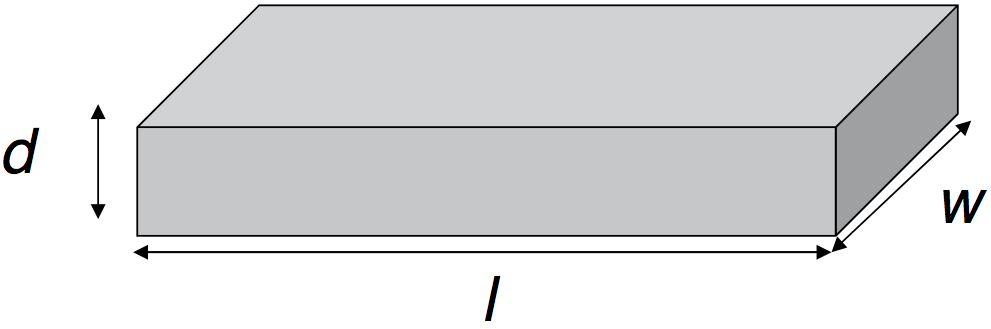
\includegraphics[scale=0.5]{pictures/widerstand}
\end{figure}
\begin{equation}
R=\rho\frac{l}{w*d}
\end{equation}
$\rho$: Spezifischer Widerstand

\subsubsection{Werte-Reihen}
\begin{itemize}
  \item E6 (1., 3., 5., 7., 9., 11. Wert der oberen Reihe)
  \item E12 (obere Reihe)
  \item E24 (obere und untere Reihe)\\
  10 12 15 18 22 27 33 39 47 56 68 82 11  13 16 20 24 30 36 43 51 62 75 91
  \item E48: Je ein Zwischenwert zu E24
  \item E96: Je ein Zwischenwert zu E48
\end{itemize}

\subsubsection{Farbcodierung}
\begin{figure}[htbs]
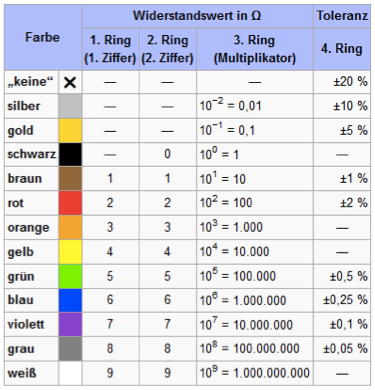
\includegraphics[scale=0.5]{pictures/farbcodierung4}
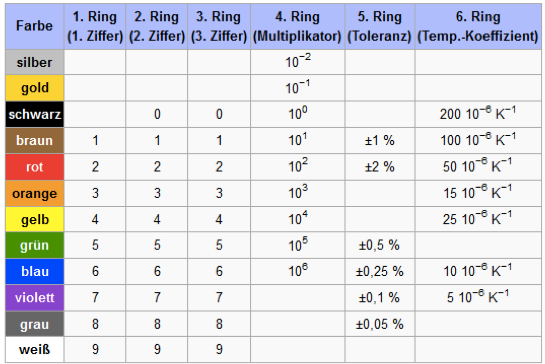
\includegraphics[scale=0.5]{pictures/farbcodierung6}
\end{figure}
\newpage
\subsubsection{SMD-Widerstände}
\begin{longtable}{|l|l|l|}
\hline
\textbf{Bauform}&\textbf{max. Verlustleistung [W]}&\textbf{max. Spannung [V]}\\
\hline
\hline
2512&1&500\\
\hline
2010&0,75&400\\
\hline
1218&1&200\\
\hline
1210&0,5&200\\
\hline
1206&0,25&200\\
\hline
0805&0,125&150\\
\hline
0603&0,1&75\\
\hline
0402&0,063&50\\
\hline
0201&0,05&30\\
\hline
01005&0,03&\\
\hline
MICRO-MELF(0102)&0,3&150\\
\hline
MINI-MELF(0204)&0,4&200\\
\hline
MELF(0207)&1&300\\
\hline
\end{longtable}

\begin{itemize}
  \item Toleranzklasse $>=$ 5\%
  \begin{itemize}
    \item zwei Ziffern für Widerstandswert
    \item Eine Ziffer für Zehnerpotenz
    \item $472=47*102 =47*100=4700\Omega=4,7k\Omega$
    \item $104=10*104 =10*10000=100.000\Omega=100k\Omega$
    \item Für Werte unter $10 \Omega$ ersetzt 'R' den Dezimalpunkt: $1R0 =
    1,0\Omega$
   \end{itemize}
   \item Toleranzklasse $< 5$\% (E48, E96)
   \begin{itemize}
     \item Drei Ziffern für Widerstandswert
     \item Eine Ziffer für Zehnerpotenz
     \item $1002=100*102 =100*100=10.000=10k\Omega$
     \item $1003=100*103 =100*1000=100.000=100k\Omega$
     \item Für Werte unter $100\Omega$ersetzt ein „R“ den Dezimalpunkt: $10R0 =
     10,0\Omega$
    \end{itemize}
\end{itemize}
\newpage
\subsubsection{Temperaturabhängige Widerstände}
\textbf{Thermistoren} sind Widerstände mit einer gezielt ausgeprägten
Temperaturabhängigkeit.\\Man unterscheidet:
\begin{itemize}
  \item PTC-Widerstände (Kaltleiter, positiver Temperaturkoeffizient): der
  Widerstandswert steigt mit steigender Temperatur
  \begin{itemize}
    \item verwendet als Temperatursensor
    \item als selbstrückstellende Sicherung
    \item als selbstregelndes Heizelement
    \item und zur Steuerung der Entmagnetisierung von Bildröhren
  \end{itemize}
  \item NTC-Widerstände (Heissleiter, negativer Temperaturkoeffizient): der
  Widerstandswert sinkt mit steigender Temperatur
  \begin{itemize}
    \item verwendet unter anderem als Temperatursensor
    \item und zur Einschaltstrombegrenzung
  \end{itemize}
\end{itemize}

\textbf{PTC}\\
\begin{figure}[htbs]
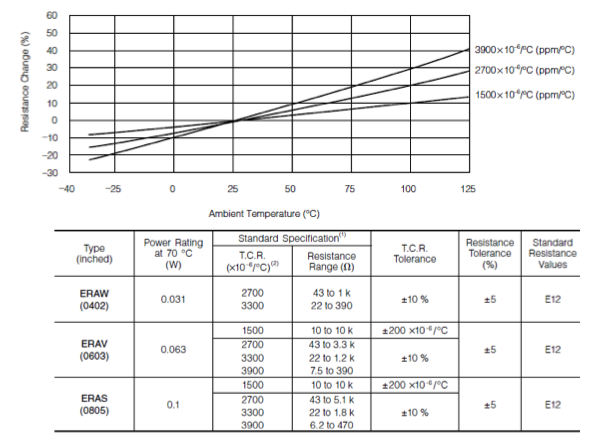
\includegraphics[scale=0.5]{pictures/ptc}
\end{figure}

\textbf{NTC}\\
\begin{minipage}{9cm}
\begin{equation}
R_{T}=R_{R}*e^{B*(\frac{1}{T}-\frac{1}{T_{R}})}
\end{equation}
\begin{tabular}{ll}
  $R_{T}$: &NTC resistance at temperature T in K\\
  $R_{R}$: &NTC resistance at rated temperature TR in K\\
  T: &Temperature in K\\
  $T_{R}$: &Rated temperature in K\\
  B: &B value, material-specific constant of NTC thermistor\\
  e: &Euler number (e = 2.71828)
\end{tabular}
\end{minipage}
\begin{minipage}{9cm}
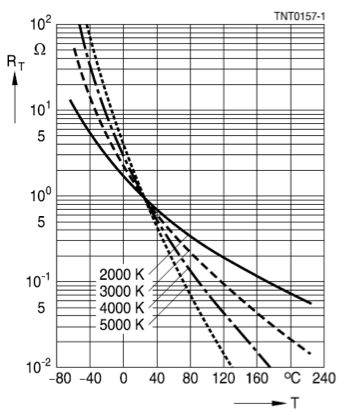
\includegraphics[scale=0.5]{pictures/ntc}
\end{minipage}

\subsubsection{Fotowiderstände}
\begin{itemize}
  \item CdS-Fotowiderstand; die fotoempfindliche Widerstandsschicht befindet
  sich zwischen den kammartigen Kontaktflächen
  \item Ein Fotowiderstand ändert seinen Widerstand unter Lichteinwirkung.
  Trifft Licht auf die fotoempfindliche Fläche des Fotowiderstands, verringert
  sich der Widerstand durch den inneren fotoelektrischen Effekt.
\end{itemize}

\subsubsection{Spannungsabhängige Widerstände}
\begin{itemize}
  \item Sie werden Varistoren (ein aus „variabel“ und „Resistor“ gebildetes
  Kunstwort) genannt und bestehen aus Metalloxiden (meist dotiertes Zinkoxid).
  \item Sie verringern ihren Widerstandswert bei steigender Spannung, meist
  drastisch ab einer charakteristischen Schwellspannung ähnlich einer
  Zener-Diode (jedoch für beide Polariäten).
  \item Sie werden zur Begrenzung von Überspannungsimpulsen (Schwellspannungen
  von 5 Volt bis mehrere Kilovolt) eingesetzt, nicht jedoch zur Spannungsstabilisierung.
\end{itemize}

\subsubsection{Druck- und dehnungsabhängige Widerstände}
\begin{itemize}
  \item Dehnmessstreifen sind Folienwiderstände, die aufgeklebt werden. Sie
  ändern ihren Widerstandswert in Abhängigkeit ihrer Dehnung beziehungsweise
  Zugspannung.
\end{itemize}

\subsubsection{Verstellbare Widerstände, Potentiometer}
\begin{itemize}
  \item Potentiometer sind für häufiges Verstellen geeignet.
  \item ein beliebiger Widerstandswert zwischen zwei Grenzwerten einstellen
  \item Trimmpotentiometer (geringe Leistung) und Stellwiderstände (grosse
  Leistung) sind nur für gelegentliches Verstellen geeignet.
\end{itemize}

\newpage
\subsection{Kondensatoren}
\begin{figure}[h]
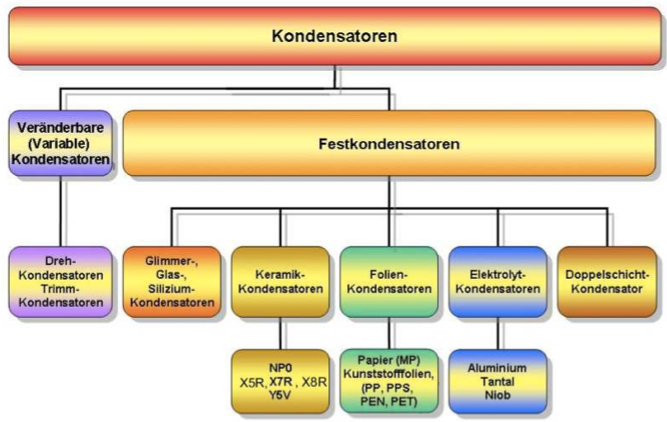
\includegraphics[scale=0.4]{pictures/kondensatortypen}
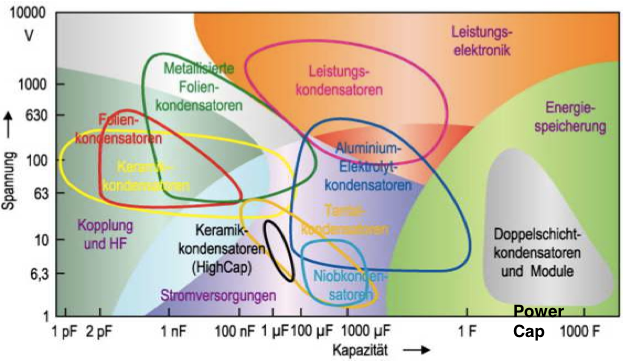
\includegraphics[scale=0.4]{pictures/spannungkondensator}
\end{figure}

\subsubsection{Kapazitätswert}
\begin{minipage}{9cm}
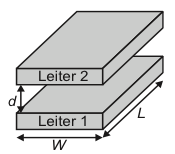
\includegraphics[scale=0.8]{pictures/kapazitaetswert}
\end{minipage}
\begin{minipage}{9cm}
\begin{equation}
C=\varepsilon_{r}*\varepsilon_{0}*\frac{W*L}{d}=\varepsilon_{r}*\varepsilon_{0}*\frac{A}{d}
\end{equation}
$\text{mit } \varepsilon_{0}= 8.85 pF/m$
\end{minipage}

\subsubsection{Anwendungsgebiete}
\begin{longtable}{|l|l|}
\hline
\begin{minipage}{4cm}
\textbf{Keramik}
\end{minipage}
&
\begin{minipage}{6cm}
\begin{itemize}
  \item Konkurrenzlos bei hohen Frequenzen
  \item Werte bis 100uF
  \item Wichtigste Anwendung: Abblockkondensatoren bei IC-Speisung
\end{itemize}
\end{minipage}
\\
\hline
\begin{minipage}{4cm}
\textbf{Tantal, EL-Elko}
\end{minipage}
&
\begin{minipage}{6cm}
\begin{itemize}
  \item Polarisiert
  \item Einsatz v.a. bei Netzteilen
  \item Stützen von Speisung und Referenzspannungen
\end{itemize}
\end{minipage}
\\
\hline
\begin{minipage}{4cm}
\textbf{Film}
\end{minipage}
&
\begin{minipage}{6cm}
\begin{itemize}
  \item Filteranwendungen
\end{itemize}
\end{minipage}
\\
\hline
\end{longtable}

\subsection{Induktivitäten/Spulen}
\subsection{Induktivität}
\begin{minipage}{9cm}
\begin{itemize}
  \item Eine Änderung des elektrischen Stromes erzeugt ein Magnetfeld, das der
  Stromänderung entgegenwirkt
  \item Masseinheit: Henry=AS/Vm
  \begin{gather}
  u_{i}=-N*\frac{d\Phi}{dt}\\
  L=\frac{N*\Phi}{I}
  \end{gather}
\end{itemize}
\end{minipage}
\begin{minipage}{9cm}
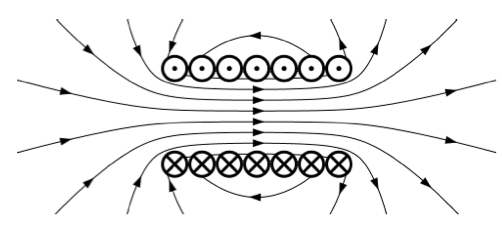
\includegraphics[scale=0.4]{pictures/induktivitaet}
\end{minipage}
\\
\begin{minipage}{9cm}
Ringspule\\
\begin{equation}
L=N^2*\frac{\mu_{0}\mu_{r}A}{2\pi r}
\end{equation}
\end{minipage}
\begin{minipage}{9cm}
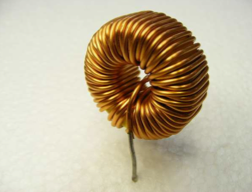
\includegraphics[scale=0.4]{pictures/ringspule}
\end{minipage}
\\
\begin{minipage}{9cm}
Zylinderspule\\
\begin{equation}
L=N^2*\frac{\mu_{0}\mu_{r}A}{l}
\end{equation}
\end{minipage}
\begin{minipage}{9cm}
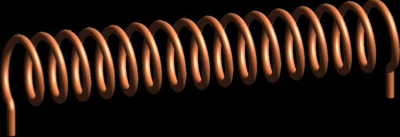
\includegraphics[scale=0.4]{pictures/zylinderspule}
\end{minipage}

\subsubsection{Einsatzgebiete und Schwerpunkte}
\begin{longtable}{|p{3.5cm}|l|l|l|l|l|}
\hline
\textbf{Application}&Inductance&Current rating&Resonance frequency&Q factor&DC
resistance\\
\hline
\textbf{RF circuits, resonant circuits}&low&low&very high&very high&low\\
\hline
\textbf{EMC}&high&high&high&low&very low\\
\hline
\textbf{RFID}&*&low&high&high&low\\
\hline
\textbf{DC/DC converters}&*&high&medium&high&low\\
\hline
\textbf{Transformers in DC/DC}&*&*&medium&*&low\\
\hline
\textbf{Signal processing}&*&low&high&-&medium\\
\hline
\end{longtable}

\subsubsection{Zusammenfassung}
\begin{itemize}
  \item Spulen sind relativ teuer
  \begin{itemize}
    \item In aktiven Filtern of durch aktive RC-Schaltungen ersetzt
  \end{itemize}
  \item Haupt-Einfastzgebiete
  \begin{itemize}
    \item DC-DC-Wandler
    \item Transformer: Galvanische Trennung
    \item Hochfrequenzanwendungen
    \item Entstörung (EMV, Datenübertragung)
  \end{itemize}
\end{itemize}
